\section{Formal Model of Hardware Wallets}\label{sec:hw_example}

Bitcoin relies on the Elliptic Curve Signature Scheme (ECDSA) for signing the
transactions and proving ownership of the assets. A Bitcoin account is defined
by a key pair $\keypair$. The public key $\pubkey$ is hashed to create an
address $\addr$ for receiving assets, while the private key $\privkey$ is used
to sign transactions that spend the assets that $\addr$ received. Unauthorized
access to $\privkey$ can result in a loss of funds, thus raising the issue of
securing the account's private keys. A Bitcoin wallet, which offers access to
the network and management of an account, is either implemented via software,
\ie is hosted online by a third party or run locally, or hardware.

The first threat arises from broken cryptographic primitives. For instance, a
broken hash function may allow an attacker to correlate an address with
multiple keys, whereas a broken signature scheme may enable an attacker to
forge transaction signatures, for addresses which it does not own.
Additionally, protecting against unauthorized access to the wallet's operations
has been shown to be as important as using secure cryptographic
primitives~\cite{SP:BMCNKF15,ISC:GkaAraKia17}. To that end, hardware wallets
offer a tamper-resistant and isolated environment for the cryptographic
primitives.

However, a hardware wallet cannot exist in a standalone setting, but rather
requires a client via which it connects to the network. Thus, if the hardware
is connected to a compromised client, any inputs/outputs of the hardware can
potentially be malicious. For example, consider Bob, whose account is defined
by the key pair $\keypair$, and an adversary $\adversary$, who is able to forge
Bob's signature. In this case any signature $\sig_{\adversary}$ of a message
$m_{\adversary}$ chosen by $\adversary$ can be verified by $\pubkey$; hence the
adversary can spend all assets that Bob has previously received, \ie the assets
sent to the hash of $\pubkey$. Let us now assume that Bob's signature is
unforgeable  but $\adversary$ controls the signing algorithm inputs, such that
for any message $m$ that Bob wishes to sign, $\adversary$ substitutes it with
$m_{\adversary}$. Even though the signature is unforgeable, the adversary can
still spend Bob's assets by tampering with the message.

Our model captures the family of attacks which tamper with the inputs/outputs
of the wallet's operations. Thus, as we show, the security of a Bitcoin
hardware wallet is reduced to the security of the underlying cryptographic
primitives \emph{and} the honesty of the three communicating parties, \ie the
hardware, the client, and the user who operates them.

We note that our model does not capture attacks on the network level. In
particular, we assume synchronous communication channels between the
participants of the hardware wallet system, \ie the user, client, and hardware;
this is a natural assumption in this setting, as we expect a direct connection
both between the client and the hardware (\eg via USB) and with the user (via
I/O devices). However, we also assume that, once a transaction is signed and
transmitted by the client, it is published on the ledger within a short time
span. Therefore, our model does not capture possible liveness violations, \eg
delays due to congestion, but rather abstracts the ledger as an ideal module
that satisfies the necessary properties. Nonetheless, a hardware wallet model
that connects to a possibly temporarily insecure ledger would be a useful
enhancement.

\paragraph{The Hardware Wallet Setting}
Software, not being tamper-resistant, cannot guarantee a secure environment for
the wallet's operations. Instead, hardware wallets offer such an environment by
separating the wallet's cryptographic primitives from the other operations, \eg
connection to the Bitcoin network. These devices do not offer network
connectivity; instead they operate in an offline mode. Due to their limited
memory capabilities and the absence of network access, they cannot keep track
of the account's activities, \eg past transactions. Thus, they connect to a
dedicated software, \emph{the client}, which records the account's actions and
provides a usable interface to the user. Hardware wallets operate under the
assumption of a malicious host and provide a trusted path with the user.
Specifically, the hardware displays transaction-related data, which the user
compares to the data presented by the (potentially compromised) client. As
such, the user becomes part of the system and is responsible for identifying
malicious actions by the client.

The wallet operations are initiated by the user, they are executed by the
client, the hardware, or both, and are as follows:
\begin{itemize}
    \item \emph{Setup}: the hardware generates a master key pair
        $\masterkeypair$ and returns the private key $\masterprivkey$, \ie the
        wallet's \emph{seed}, to the user; currently all wallets are
        Hierarchical Deterministic~\cite{CCS:DasFauLos19}, mostly based on the
        BIP32 standard~\cite{bip32}.
    \item  \emph{Session Initialization}: the hardware connects to the client
        and sends to it the master public key $\masterpubkey$;
    \item \emph{Generate Address}: both the client and the hardware generate a
        new address and return it to the user. The hardware derives a key
        pair $(\privkey_i, \pubkey_i)$ from $\masterkeypair$, generates the
        address $\addr_i$ and returns it to the user. The client may either
        generate $\pubkey_i$ using $\masterpubkey$ or receive $\pubkey_i$ from
        the hardware, then generates and stores the corresponding address, and
        finally returns it to the user.
    \item \emph{Calculate Balance}: given a list of the account's addresses,
        the client iterates over the ledger's transactions, calculates the
        account's available assets and returns this amount to the user.
    \item \emph{Transaction Issuing}: the user provides the payment data to the
        client, \ie the amount and receiver's address, which then forwards them
        to the hardware together with the available inputs, \ie the account's
        addresses and balance, and requests its signature. The hardware checks
        whether the inputs belong to the managed account and generates a
        \emph{change address} upon demand, \ie if the balance is larger than
        the payable amount. Then, it requests the user's approval of the
        payment data; if the user confirms the payment, the hardware signs it
        and returns the signature together with the corresponding public key to
        the client in order to publish it on the network.
\end{itemize}
Figure~\ref{fig:user_wallet} illustrates the issuing of a transaction in the
hardware-enhanced wallet setting.

\begin{figure}
    \begin{center}
        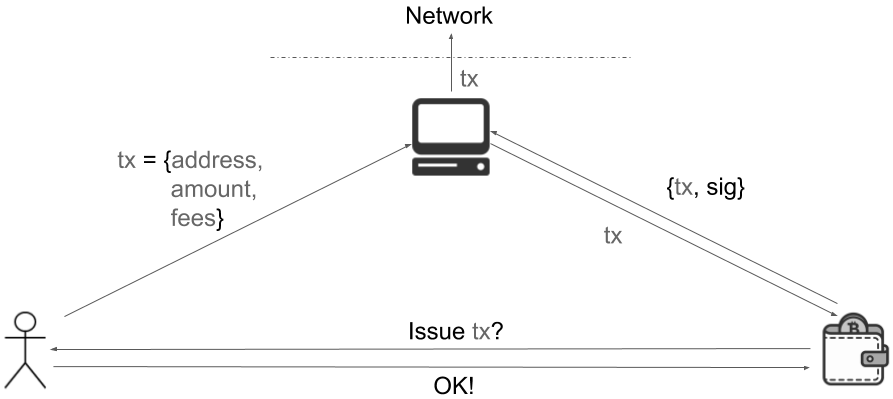
\includegraphics[width=0.75\columnwidth]{figures/hardware-wallets/user_wallet_bw.png}
    \end{center}
    \caption{Transaction issuing in the hardware wallet setting.}
    \label{fig:user_wallet}
\end{figure}

Evidently, a hardware-assisted wallet is not a single module, but rather an
``ecosystem'' of modules that communicate during an operation: the user, the
client, and the hardware. To treat it under the UC framework, we will next
describe an ideal functionality, that defines the wallet's properties, as well
as its real world implementation. In the ideal world, the wallet is a
monolithic component-functionality, responsible for all aforementioned
operations.  In the real world, the wallet emerges through the interaction of
the human operator, the client (\ie a desktop computer, tablet, or smartphone),
and a tamper resistant hardware component. To prove the security of the
real-world protocol, we will compare the two executions (in the real and ideal
settings) and show that they are indistinguishable.

\paragraph{Ideal World}
The wallet functionality, $\Fw$, defines the wallet's operations in the ideal
setting. $\Fw$ interacts with the global Bitcoin ledger functionality $\Gledg$,
as defined in~\cite{C:BMTZ17}, in order to execute operations requiring access
to the decentralized system. $\Gledg$ is the ideal functionality that models
the Bitcoin ledger and allows a wallet to register itself, publish transactions
and retrieve the state of the ledger, \ie all published transactions. $\Fw$
generates a unique address per public key and also incorporates a signature
functionality, $\Fsig$, as defined in~\cite{EPRINT:Canetti03}; for ease of
notation, we show $\Fsig$ as a separate component in the ideal world, although
in fact $\Fw$ simply repeats the steps defined in $\Fsig$. Specifically, the
wallet registers itself with $\Fsig$, which creates fresh keys for the account
upon request, \eg during address generation, and signs messages, \eg
transactions. $\Fsig$ is also accessed by the validation predicate of $\Gledg$,
in order to verify a transaction's signature during the validation stage.

\paragraph{Real World}
The operations defined by $\Fw$ are executed in the real world by a set of
communicating parties: the \emph{hardware}, the \emph{client}, and the
\emph{user}. Thus the protocols of the hardware $\Fhw$, the client $\pclient$,
and the human $\ph$ define the actions of the corresponding parties. The
hardware protocol $\Fhw$, uses a signature scheme $\Sigma \equiv \langle
\algokeygen, \algoverify, \algosign \rangle$, a cryptographic hash function
$\hash$ and a pseudorandom key generation function
$\mathsf{HierarchicalKeyGen}(\masterprivkey, i)$, in order to derive children
keys from the master key. A basic assumption of this setting is that $\pclient$
runs in an untrusted environment, \ie we do not assume the software to be
secure. Thus, in our model, connection to a malicious client is equivalent to
corruption of the client by the adversary. Finally, the user communicates with
the hardware and the client via a secure channel, \ie can interact directly
with the device via buttons and/or a display.

\paragraph{Validation Predicate}\label{sec:validation_predicate}
In both settings, $\Fw$ and the real-world parties have access to a global
Bitcoin ledger functionality $\Gledg$, as defined in~\cite{C:BMTZ17}. $\Gledg$
is parameterized with the validation predicate $\algovalidate$, which
identifies whether a transaction can be added to its buffer, \ie if it is valid
for publishing on the ledger.  The predicate takes as input the candidate
transaction, the buffer, and the current state. The transaction consists of the
signed data $\tx_\sig = (\tx, \pubkey, \sig)$ and ledger parameters, \eg the
transaction id, which is a unique identifier of the transaction, and the
timestamp, \ie the time defined by a global clock. Intuitively, the Bitcoin
state is the blockchain, while the buffer is the mempool, which contains the
transactions that have not yet been included in the blockchain. In our model,
the validation predicate performs the signature verification of a transaction.
This is formalized with a wrapper $\mathsf{ValidateWrapper}$, which wraps all
instantiations of the validation predicate. In the ideal world, the wrapper
accesses the signature functionality $\Fsig$ to verify the transaction's
signature; if the signature is not valid, then it directly outputs $0$,
otherwise it performs all additional checks, such as verifying the consumed
funds and checking the amounts' validity.  The ideal wrapper
$\mathsf{IdealValidateWrapper}$ is described in Algorithm
\ref{alg:validatewrapper}. The real-world wrapper
$\mathsf{RealValidateWrapper}$ uses a signature scheme instead of $\Fsig$ and
behaves similarly to Algorithm \ref{alg:validatewrapper}, \ie it first parses
$\mathsf{BTX}$ and then performs the same branch checks on $\algoverify(\tx,
\pubkey, \sig)$ and returns the proper boolean value.

\begin{algorithm}
    \caption{
        The validation predicate wrapper, parameterized by $\algovalidate$
        and $\Fsig$. The input is a transaction $\mathsf{BTX}$, the buffer
        $\mathsf{buffer}$ and the state $\mathsf{state}$.
    }
    \label{alg:validatewrapper}
    \begin{algorithmic}
        \Function {$\mathsf{IdealValidateWrapper}$}{$\mathsf{BTX, buffer, state}$}
            \State $(\tx, \pubkey, \sig, \msf{txid}, \tau_L, p_i) = \msf{parse}(\mathsf{BTX})$
            \State Send $\msg{Verify}{\tx, \sig, \pubkey}$ to $\Fsig$ and receive $\msg{Verified}{\tx, f}$
            \State \Return $f$
        \EndFunction
    \end{algorithmic}
\end{algorithm}

Finally, Figure~\ref{fig:wallet_worlds} illustrates the ideal and the real
world settings.  In both worlds, the environment $\env$ interacts with the
adversary; Specifically, in the ideal world it interacts with the simulator
$\simulator$ and in the real world with the adversary $\adversary$. In the
ideal world, the wallet consists of the ideal wallet functionality $\Fw$ and
the signature functionality $\Fsig$. In the real world, it consists of the
user, client, and hardware parties, who execute the respective protocols $\ph,
\pclient, \Fhw$.  Communication between the human, client, and hardware is
achieved over a \emph{UC-secure channel protocol}, as presented by
Canetti~\cite{EPRINT:CanKra02a}. Specifically, the adversary is able to observe
the encrypted communication between the honest parties, but can only retrieve
the length of the exchanged messages and not tamper with the plaintext. In
practice, this can be achieved by establishing a secure channel between the
client and the hardware module using standard key exchange techniques, while
the human-hardware channel is assumed to be secure by default. We note that, in
the absence of a secure channel, the adversary may tamper with the
communication, so, in our model, an insecure channel is equivalent to the
client being corrupted.

\begin{figure}
    \begin{center}
        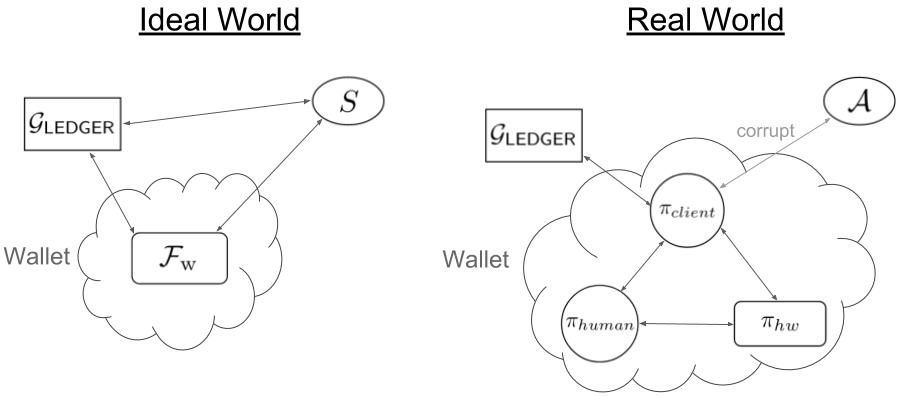
\includegraphics[width=0.80\columnwidth]{figures/hardware-wallets/worlds_bw.png}
    \end{center}
    \caption{A high-level comparison of the ideal and the real worlds.}
    \label{fig:wallet_worlds}
\end{figure}

In the chapter's upcoming sections we use a simplified transaction model, for
ease of notation. Specifically, each transaction defines a single input and
output. We note that adapting it for multiple inputs and outputs, in order to
properly model real-world ledgers, is rather straightforward. The wallet's key
pairs, and consequently its addresses, are generated using the master key pair
$\masterkeypair$, which is randomly selected from the key domain $\keyset$ upon
the wallet's setup. Following, the addresses' keys are derived from a master
key pair as $\privkey_i = \masterprivkey + \hash(i, \masterpubkey)(\bmod$ $n)$
and $\pubkey_i = \masterpubkey + \hash(i, \masterpubkey) \times N$, where $i$
is the index of an address and $n, N$ are public parameters of the Elliptic
Curve. A hardware wallet transaction is a tuple $\tx = (\addr_\msf{s},
\addr_\msf{r}, \asset_\msf{pay}, \addr_\msf{c},
\asset_\msf{change})$. Specifically, $\addr_\msf{s}$ denotes the sender's
address, $\addr_\msf{r}$ the receiver's address, and $\addr_\msf{c}$ the
change address. Additionally, $\asset_\msf{pay}$, $\asset_\msf{change}$
$\asset_\msf{fee}$ are the payment, change and fee funds respectively;
notably, $\asset_\msf{change}$ equals to the account's balance minus the
payment and the fee amounts, \ie $\asset_\msf{change} =
\textrm{balanceOf}(\addr_\msf{s}) - \asset_\msf{pay} -
\asset_\msf{fee}$. A signed transaction is the tuple $(\tx, \pubkey, \sig)$,
where $\sig$ is the signature of $\tx$ under the public key $\pubkey$.  The
parties that execute an operation are the user $\user$, \ie the owner of the
wallet, the client $\client$, \ie the device to which the hardware connects,
and the hardware $\hardware$. Each message is associated with a session id
$\sid' = \user\client\hardware$, which defines the parties with which it is
related.
